\subsubsection {Búsqueda tabú}
Sus orígenes se atribuyen a mediados de los 60 y 70 por Fred Glover (\cite{ [GLOVER]}), la búsqueda tabú se encarga de evitar caer en soluciones comunes evitando ciertos movimientos, clasificándolos como tabú. El propósito de clasificarlos es evitar que se repitan los mismos resultados durante la búsqueda, ya que los movimientos prohibidos constituye solo una parte del total de movimientos disponibles.\\
\hspace*{1cm}La premisa de la búsqueda tabú es la de emular el mecanismo de intuición natural para tomar decisiones, proceso en el cual se introduce uno o varios elementos aleatorios, que puede llegar a concluir desde soluciones poco prácticas o erróneas, o traer una mejor solución. Al emular este mecanismo se elige cualquier movimiento sin importar que traiga la peor solución, a excepción que el movimiento seleccionado recorra una ruta similar a las ya examinadas previamente. Con estas condiciones, la técnica buscará el mejor movimiento posible, aun así la búsqueda regresara al estado inicial para seguir buscando desde otro ángulo. Para ello, se mantiene información referente a los movimientos más recientes en segmentos de memoria (también llamados listas tabú), para evitar que recorra una ruta ya examinada previamente, aunque esta prohibición es generalmente condicional y no absoluta.\\
\hspace*{1cm}En la figura \ref{fig:iteration} se puede ver que se empieza con una solución, la cual a partir de ésta se crean nuevas soluciones que se derivan de la misma, la solución que cumpla con las características de admisibilidad o no (dependiendo de que existan otros criterios) se irán agregando a una lista de soluciones admisibles, la mejor será la que tomará el rol de la solución óptima y se repetirá el ciclo hasta que el usuario lo permita, al final se tomará toda la lista de admisibles junto con la mejor como resultado.

    \begin{figure}[hbtp]
        \centering
            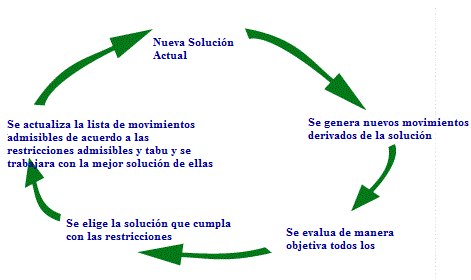
\includegraphics[width=0.5\textwidth]{MarcoTeorico/Imagenes/iteration.png}
            \caption{Resumen de como funciona la búsqueda Tabú.}                       
            \label{fig:iteration}
    \end{figure} 
    
Resumiendo, la búsqueda tabú tiene 3 conceptos principales:

\begin{itemize}
\item \textbf{Memoria de corto y largo plazo: } Estos segmentos de memoria se encargan de guardar varias listas, una de corto plazo para movimientos plausibles (que se derivan de una solución) y otra de largo plazo que guarda una lista de movimientos admisibles donde entran todas las soluciones que hayan cumplido con los criterios requeridos.
\item \textbf {Mecánica de admisibilidad: } Para evitar que cualquier solución entre a la lista de admisibles debe de existir un conjunto de normas para comprobar si es tabú o no, esta mecánica debe de irse cambiando conforme avanza el proceso.
\item \textbf {Una mejor solución global: } Aunque se vayan generando diversas soluciones, la solución óptima sera la definitiva.
\end{itemize}

\hspace*{1cm}El código \ref{lst:busquedatabu} representa una versión general del algoritmo de búsqueda tabú:\\

\begin{lstlisting}[language=HTML, caption=Búsqueda tabú, label=lst:busquedatabu]
Mejor Solución = Solución Inicial;

    Mientras (¿Cumple con los criterios de continuación?){
      Lista  de movimientos plausibles(soluciones derivadas de la mejor solución)
      Mientras(¿Hay mas  elementos de la lista de movimientos por revisar?){
    	Seleccionar una solución de la lista;
    	Si(solución seleccionada>mejor solución plausible){
     	  Si(¿Cumple con las restricciones tabú?){
    		Si(Cumple con los criterios de admisibilidad){
    			Entra a la lista de admisibles ;
    		}
    	  }No : Entra a la lista de admisibles ; 
    	}
      }
    
      Si(Mejor Solución plausible> Mejor Solución Global){
         Mejor Solución Global = Mejor Solución Plausible;
      }
    
      Si(Cumple con los criterios de continuación){
    	Solución Inicial = seleccionar cualquiera de la lista de soluciones admisibles;
    	Actualizar criterios tabú y admisibles;
      }
    }
    
    Retornar Mejor Solución Global;
Fin;
\end{lstlisting}